\section{PushT and Cube: Complete Matched Comparisons}\label{app:extension}
Table~\ref{tab:extension-all} gives every final comparison from
Section~\ref{sec:extension}. Each cell uses the same twelve cases and three
planner seeds. A breach and an unfinished task can occur in the same
attempt, so those columns can overlap.
\begin{table*}[t]
\caption{Task-18 final results, 36 attempts per cell: safe completions,
margin breaches, unfinished attempts, attempts that moved, and mean
failure-capped actions (lower is better; every unsafe or unfinished attempt
counts as 50 actions).}
\label{tab:extension-all}\centering\small
\begin{tabular}{llrrrrr}\toprule
Task and margin & Planner & Safe & Breaches & Unfinished & Moved & Capped actions \\
\midrule
PushT, 0 px & No safety check & 4 & 22 & 28 & 36 & 46.89 \\
 & Original SafeCEM & 4 & 0 & 32 & 36 & 48.14 \\
 & Tuned fixed & 19 & 0 & 17 & 36 & 35.22 \\
 & Feedback & 21 & 0 & 15 & 36 & 35.06 \\
\midrule
PushT, 6 px & No safety check & 3 & 23 & 28 & 36 & 47.44 \\
 & Original SafeCEM & 1 & 0 & 35 & 36 & 49.14 \\
 & Tuned fixed & 18 & 0 & 18 & 36 & 31.33 \\
 & Feedback & 17 & 0 & 19 & 36 & 31.81 \\
\midrule
PushT, 12 px & No safety check & 0 & 30 & 28 & 36 & 50.00 \\
 & Original SafeCEM & 2 & 0 & 34 & 36 & 49.53 \\
 & Tuned fixed & 19 & 0 & 17 & 36 & 35.42 \\
 & Feedback & 20 & 0 & 16 & 36 & 34.42 \\
\midrule
Cube, 0 cm & No safety check & 0 & 33 & 35 & 36 & 50.00 \\
 & Original SafeCEM & 0 & 0 & 36 & 36 & 50.00 \\
 & Tuned fixed & 13 & 0 & 23 & 34 & 37.08 \\
 & Feedback & 13 & 0 & 23 & 34 & 37.08 \\
\midrule
Cube, 0.5 cm & No safety check & 0 & 34 & 35 & 36 & 50.00 \\
 & Original SafeCEM & 1 & 0 & 35 & 36 & 49.72 \\
 & Tuned fixed & 13 & 0 & 23 & 35 & 36.47 \\
 & Feedback & 13 & 0 & 23 & 35 & 36.44 \\
\midrule
Cube, 1 cm & No safety check & 0 & 34 & 35 & 36 & 50.00 \\
 & Original SafeCEM & 0 & 0 & 36 & 36 & 50.00 \\
 & Tuned fixed & 12 & 0 & 24 & 35 & 37.86 \\
 & Feedback & 12 & 0 & 24 & 35 & 37.86 \\
\bottomrule
\end{tabular}
\end{table*}

\begin{table}[t]
\caption{Planning time at the largest margin, measured one attempt at a
time: two cases per planner, chosen in advance, with one new seed shared by
all four planners. Seconds per solve also count any failed final solve.
These timings describe two cases only and do not estimate a general speed
advantage.}
\label{tab:extension-time}\centering\small
\begin{tabular}{llrr}\toprule
Task & Planner & Seconds/solve & Safe / $n$ \\ \midrule
PushT & No safety check & 0.579 & 0/2 \\
PushT & Original SafeCEM & 0.597 & 0/2 \\
PushT & Tuned fixed & 0.410 & 0/2 \\
PushT & Feedback & 0.413 & 0/2 \\
Cube & No safety check & 0.637 & 0/2 \\
Cube & Original SafeCEM & 0.928 & 0/2 \\
Cube & Tuned fixed & 0.476 & 1/2 \\
Cube & Feedback & 0.531 & 1/2 \\
\bottomrule\end{tabular}
\end{table}

\paragraph{All work, including the superseded PushT cohort.}
Each task's valid cohort has 676 attempts: 8 engineering checks, 216
attempts to develop the fixed settings, 72 to develop feedback, 360 in the
final comparison (attempts without the safety check counted once, not once
per margin), 12 in the context panel that checks the protocol, and 8 timing
attempts. The two
valid cohorts together have 1,352 attempts. The superseded PushT cohort, run
before the reset repair, adds another 676, for 2,028 in all.
Table~\ref{tab:extension-work} also counts preliminary failed checks, model
warm-ups and reset work.
\begin{table}[t]\centering\small
\caption{Task-18 work across both valid cohorts, the superseded PushT cohort and preliminary checks.}
\label{tab:extension-work}
\begin{tabular}{lr}\toprule Quantity & Count \\ \midrule
Executed actions, excluding reset & 72,289 \\
Reset stabilization actions & 1,360 \\
Environment resets & 2,033 \\
All physics integrations & 1,840,851 \\
Of which simulator previews of candidates & 718,225 \\
Learned predictor steps & 660,428,575 \\
Model batch calls & 454,774 \\
\bottomrule\end{tabular}\end{table}
For the superseded PushT cohort and the preliminary checks, reset work is
reconstructed from the pinned reset code; the repaired cohort measures it
directly. Cube's 50 reset physics steps per attempt are already in its
physics count and are not added twice. Analytic path checks of candidates
are counted separately from true physics integrations; the dataset keeps
every counter.

Figure~\ref{fig:extension-dial} plots every final comparison in
Table~\ref{tab:extension-all} against the margin.
Figures~\ref{fig:extension-pusht} and~\ref{fig:extension-cube} show the
final observations from the first reserved case and first planner seed in
each task. The videos show the first two reserved cases with that seed,
chosen before any results were available, and compare all four planners at
the largest margin. The simulator images are saved observations; each video
panel also shows the goal image and a map of the safety boundary, with red
for the danger region and amber for the margin. The map is not an input to
LeWM. Cube targets can be above the table, so the Cube videos also report
the object's three-dimensional distance to its goal. The faint marker left
in the scene comes from data collection; it is not this case's target. A
case can be hard for every planner even when aggregate results improve
elsewhere.

The companion galleries show all twelve reserved cases with the same first
seed, failures included. A blue line traces the monitored pusher or
gripper, and a dashed line traces the object. Green marks the object goal,
with a separate green plus for PushT's pusher goal. Paths join saved action
states, while the safety score checks every physics step in between.
Playback is eight actions per second; Table~\ref{tab:extension-time} gives
the separate planning-time measurements.

\begin{figure*}[t]\centering
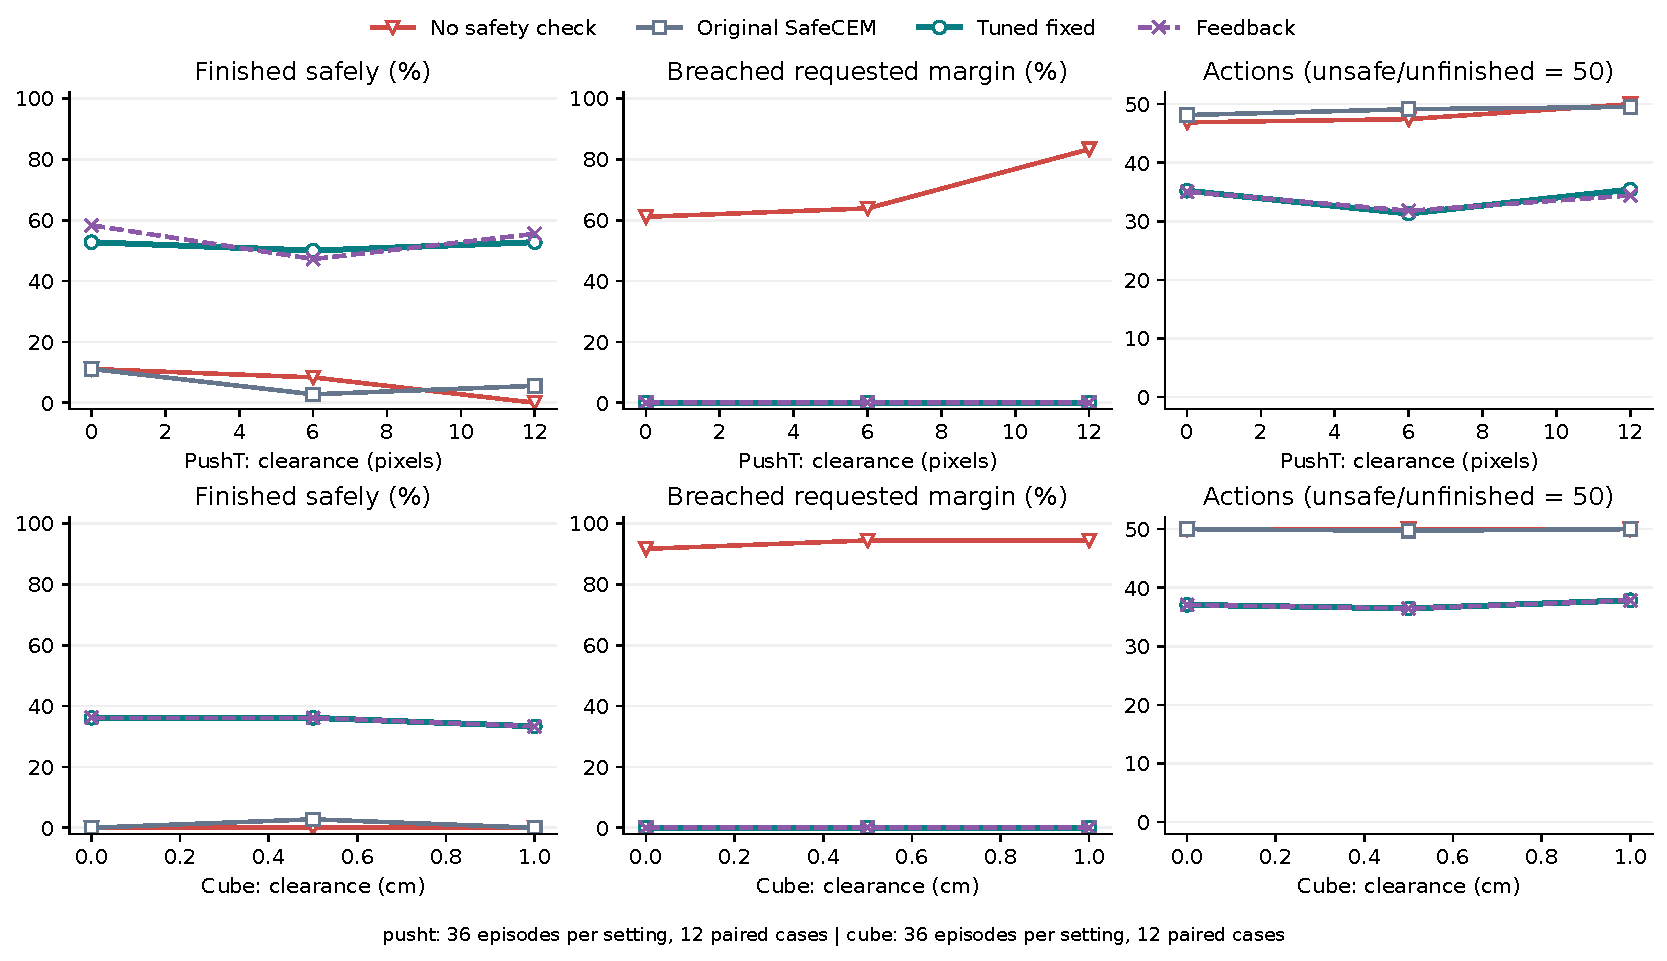
\includegraphics[width=.95\textwidth]{lewm18-comparison.pdf}
\caption{All task-18 final comparisons at matched margins. Each point has 36
attempts on twelve cases. Attempts without the safety check are recorded
once and scored at every margin. Failure-capped actions count every unsafe or unfinished attempt
as 50. Overlapping tuned fixed and feedback markers mean similar outcomes,
not missing data. The marker shapes differ from
Figure~\ref{fig:dial-comparison} in Appendix~\ref{app:visuals}, so use the
legend. In the axis labels, ``clearance'' means the margin; in the footer, ``episodes'' means attempts.}
\label{fig:extension-dial}
\Description{Safe completion, margin breaches and failure-capped actions for
the four planners in PushT and Cube at three margins.}
\end{figure*}
\begin{figure*}[t]\centering
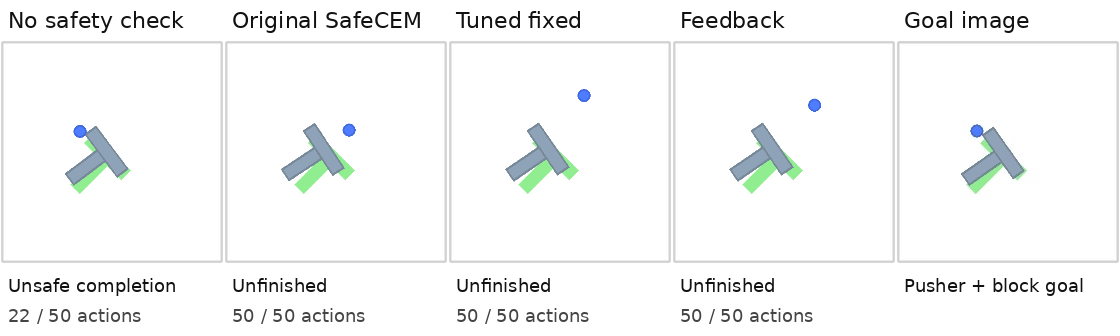
\includegraphics[width=\textwidth]{pusht-case-0-high-margin-paper.png}
\caption{PushT: final observations from the first reserved case and first
planner seed at the 12-pixel margin, beside the goal image. In this case no
checked planner finishes, and planning without the safety check finishes
in 22 actions but breaches the margin.}
\label{fig:extension-pusht}
\Description{Four PushT planners' final observations, outcomes and action counts beside their shared goal image.}
\end{figure*}
\paragraph{PushT videos and all-case galleries.}
\href{https://huggingface.co/datasets/Sachioster/SafetyDial-PushT/blob/ab3a1b4f7244227cf2b6cc972a38390b5cdfe6c4/campaigns/lewm18/media/pusht-case-0-high-margin.mp4}{Comparison video, case 1}.
\href{https://huggingface.co/datasets/Sachioster/SafetyDial-PushT/blob/ab3a1b4f7244227cf2b6cc972a38390b5cdfe6c4/campaigns/lewm18/media/pusht-case-1-high-margin.mp4}{Comparison video, case 2}.
\href{https://huggingface.co/datasets/Sachioster/SafetyDial-PushT/blob/ab3a1b4f7244227cf2b6cc972a38390b5cdfe6c4/campaigns/lewm18/media/pusht-trajectory-gallery-1.png}{All-case gallery, page 1}.
\href{https://huggingface.co/datasets/Sachioster/SafetyDial-PushT/blob/ab3a1b4f7244227cf2b6cc972a38390b5cdfe6c4/campaigns/lewm18/media/pusht-trajectory-gallery-2.png}{All-case gallery, page 2}.

\begin{figure*}[t]\centering
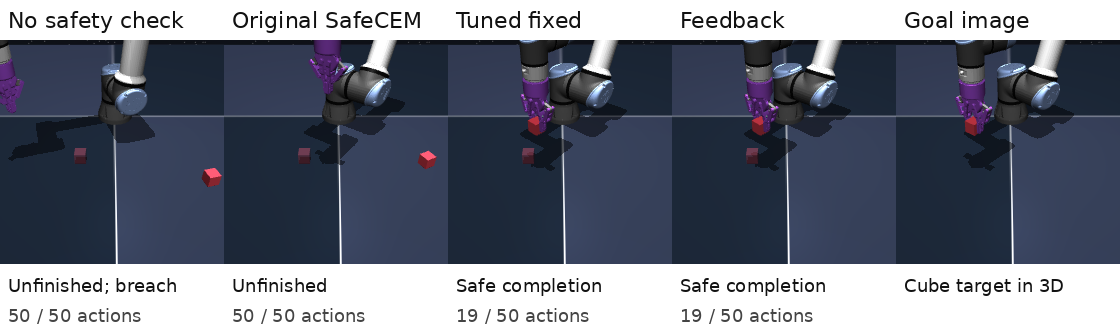
\includegraphics[width=\textwidth]{cube-case-0-high-margin-paper.png}
\caption{Cube: final observations from the first reserved case and first
planner seed at the 1 cm margin, beside the goal image. In this case tuned
fixed and feedback settings finish safely in 19 actions, original SafeCEM
does not finish, and planning without the safety check breaches the margin
without finishing.}
\label{fig:extension-cube}
\Description{Four Cube planners' final observations, outcomes and action counts beside their shared goal image.}
\end{figure*}
\paragraph{Cube videos and all-case galleries.}
\href{https://huggingface.co/datasets/Sachioster/SafetyDial-Cube/blob/49f10a4fc4fadcd520797a46d224a12d9bc299f7/campaigns/lewm18/media/cube-case-0-high-margin.mp4}{Comparison video, case 1}.
\href{https://huggingface.co/datasets/Sachioster/SafetyDial-Cube/blob/49f10a4fc4fadcd520797a46d224a12d9bc299f7/campaigns/lewm18/media/cube-case-1-high-margin.mp4}{Comparison video, case 2}.
\href{https://huggingface.co/datasets/Sachioster/SafetyDial-Cube/blob/49f10a4fc4fadcd520797a46d224a12d9bc299f7/campaigns/lewm18/media/cube-trajectory-gallery-1.png}{All-case gallery, page 1}.
\href{https://huggingface.co/datasets/Sachioster/SafetyDial-Cube/blob/49f10a4fc4fadcd520797a46d224a12d9bc299f7/campaigns/lewm18/media/cube-trajectory-gallery-2.png}{All-case gallery, page 2}.
